\documentclass{eusflat2019}

\usepackage{amsmath,amssymb}
\usepackage{csquotes}
\usepackage{graphicx}
\usepackage[colorlinks=true]{hyperref}
\usepackage{array}
\usepackage[export]{adjustbox}
\usepackage{subcaption}
\usepackage{fancyhdr}
\usepackage{lastpage}

\title{\bf Exploring Lagrangian Coherent Structures in Boids-like Simulations of Isolated Ant Colonies}

\renewcommand\vec{\mathbf}

\author{{\bf Parth Sastry}\\
Undergraduate, Department of Physics, Indian Institute of Technology - Bombay \\ parth.sastry@iitb.ac.in}

\begin{document}
\maketitle
\begin{abstract}
\textit{Taxis} is the movement of organisms in response to stimuli like light, sound, food presence, etc. The primary driver of ant movement is \textit{chemotaxis}, where ants get directed by the concentration gradient of pheromones they deposit on the ground. This leads to emergent behaviour such as lane formation when foraging, and in rare cases, formation of large circular ant mills when ants are moved to a new environment. We try to model the movement of individual ants as a mixed random walk with memory. We then analyse the Lagrangian Coherent Structures that emerge in this motion, treating individul ants as being driven by a background 'flow'.

{\bf Keywords:} Chemotaxis, Random Walks, Lagrangian Coherent Structures
\end{abstract}

\section{Introduction}
\label{section:intro}
\subsection{Biological Background}
Chemotaxis (from the stem of “chemistry” and Gr. $\tau\acute{\alpha}\xi\iota\varsigma$, arrangement), is a biological term for the attraction exercised on living or growing organisms or their members by chemical substances \cite{chemotaxisEncyclopedia}. As an example, during the expansion of a tumour, formation of new blood vessels, known as \textit{angiogenesis}, also involves chemotaxis. Chemical agents secreted by a tumor attract neighboring endothelial cells. These cells form the surface of blood vessels which provide nourishment to the tumour. \cite{MPlank:Angiogenesis}\cite{FriedmanTello2002}

Ants communicate with each other using pheromones, sounds, and touch \cite{Jackson2006}. They perceive smells via their antennae and leave pheromone trails on the ground where they may be followed by other ants. This is notably seen in foraging parties. When a forager ant finds food, it marks a trail on the way back to the colony, which is reinforced when other ants follow the previous trail and head back with food to the colony. \cite{Goss1989}

This is chemotaxis driven not by external chemical gradients, but by chemicals laid down by other individual entites, which makes the motion of ants interesting to study. Some questions to ask are - can ant motion be fully explained by chemotactic stimuli? Do ants, like birds or fish schools, form larger subgroups and tend to follow other ants? We explore these questions and try to analyse the dynamics that arise when incorporating stimuli other than chemotaxis. See Section \ref{Section:Schooling}

\subsection{Mathematical Background}
Analysing the movement of individual entities driven by chemotaxis, as being driven by a background flow (analogous to particles being carried by a fluid flow), alllows us to comment on the underlying dynamics of the flow. This is where Lagrangian Coherent Structures come in. The theory is discussed further in Section \ref{section:LCS} and the the emergent LCSs seen in the results of our simulation are discussed.

The mathematical description of bodies whose motion is dictated by chemotaxis is given by reinforced random walks (RRWs). A random walk is a mathematical object describing a path characterized by succession of random steps over some space (in our case, the position space). In RRWs, paths followed by individuals can be \textit{reinforced}, as in the case of motion of ants which reinforce trails by laying down pheromone. RRWs have been extensively used to model observed chemotaxis phenomena \cite{Codling2008}\cite{Pemantle2007}.

In her 2017 paper, Ria Das extends the models given by Codling, Plank and Benhamou \cite{Codling2008} to account for the inertia of biological entities to continue moving in their direction of motion, resisting changes in velocity \cite{RiaDas2017}. They construct a continuous random walk model based on diffusion-advection partial differential equations that combine memory and reinforcement. The basis for their system  is a pair of pure reinforcement equations for the particle density and chemical concentration in a  one-dimensional environment from Othmer and Stevens \cite{Stevens1997}. 

\subsection{Combining Multiple Models}
In their 2002 paper, Iain Couzin and Nigel Franks developed a set of movement rules of individual ants on trails that lead to a collective choice of direction
and the formation of distinct traffic lanes that minimize congestion \cite{Couzin2003}. The general principle of turning towards a positive pheromone concentration gradient is common across the continuous model given by Ria Das and the model given by Couzin and Franks.

They differ in that Couzin and Franks were modelling the propensity of ants to follow a pre-existing trail and align their directions to each other. Ria Das also tries to incorporate pheromone deposition in their continuous random walk model.

We try to combine the rules of motion of individual ants given by Couzin and Franks, with the more real-world nature of how trails form - by continuous deposition and evaporation of pheromone along the positions of the ants.


\section{Model}
\label{section:model}
Interaction of ants with the pheromone deposited on the ground, and with other ants is taken from Couzin and Franks' 2002 paper \cite{Couzin2003}. To simulate pheromone deposition and evaporation, we take ideas from Ria Das' paper, and apply some modifications to account for discrete individuals depositing pheromone, and deposition on discrete grid points.

\subsection{Overview}
$N$ ants are simulated. We keep track of each ants' position vector $\vec{c}_i(t)$ and orientation vector $\vec{v}_i(t)$. Ant heads are at position $\vec{c}_i(t) + 1/2 \beta \vec{v}_i(t)$, where $\beta = 0.8cm$ is the ant body length. The left and right antennae each extend a distance $\phi = 0.4cm$ from the head at an angle of $45^\circ$ to the ant’s body orientation. In the simulation, ants will turn away from others if they are approached too closely within either of two local areas. 

\begin{enumerate}
    \item The first is a circle, radius $r_d = 0.4 cm$, extending from the ant’s centre, $\vec{c}_i(t)$, representing very close proximity to the body and legs of the ant.
    \item The second is an arc that extends ahead of the ant a distance $r_p = 1.2 cm$ from $\vec{c}_i(t)$ and has an internal angle $\alpha$ (taken to be $90^\circ$ for the simulations); this may represent a local visual field or tactile range of the antennae
\end{enumerate} 

Individuals tend to turn away from others within these zones with a turning rate $\theta_a = 1000^\circ \, s^{-1}$. When not avoiding collisions, ants respond to local concentrations of pheromone.

Ants turn towards the highest stimulus (perceived pheromone concentration) at turning rate $\theta_p = 500^\circ \, s^{-1}$. When ants are not avoiding collisions they accelerate with acceleration $\mu = 50 cm \, s^{-2}$ until they reach their desired speed $u_{des} = 13 cm \, s^{-1}$.

Time is simulated via discrete steps of $0.02 s$ each. At each time-step, the direction vectors and then the position vectors of all ants are updated in parallel.

\subsection{Inter-Ant Interaction}

If there are ants $j$ within the interaction zone (specified above) of ant $i$, ant $i$ turns away from them by turning towards a desired vector - 

\begin{equation}
    \vec{d}_i(t + \Delta t) = \sum_{j \neq i} \frac{\vec{c}_i(t) - \vec{c}_j(t)}{|\vec{c}_i(t) - \vec{c}_j(t)|}
\end{equation}

The ant can, of course, turn through a maximum of $\theta_a\Delta t$ degrees in $\Delta t$. If this angle is greater than, or equal to the angle between initial orientation $\vec{v}_i(t)$ and desired orientation $\vec{d}_i(t)$, then it matches the desired orientation. Otherwise it turns through $\theta_a\Delta t$ degrees towards the desired orientation.

\subsection{Pheromone Interaction}

Deposition of pheromone is specified in the subsection \ref{subsec:pheromone}. If there are no other ants within the interaction zones of ant $i$, it responds instead to pheromone concentration. At a given point in time, the ant samples concentrations $C_l$ and $C_r$ at the ends of the left and right antennae,
respectively. To simplify calculations, instead of converting this into a stimullus intensity and adding gaussian noise, as is specified in \cite{Couzin2003}, we simply sample the concentrations at the two antennae, and turn $\theta_p \Delta t$ degrees towards the higher concentration.

If no concentration difference is detected, the orientation doesn't change.

All turnings (inter-ant interactions, as well as pheromone interactions) are subject to turning error. This is simulated by adding Gaussian noise of mean $0$ and standard deviation $0.5 \text{rad}$ to $\vec{v}_i(t + \Delta t)$.

\subsection{Pheromone Concentration}
\label{subsec:pheromone}

This is a new feature we add to the original model derived by Couzin and Franks. In their model, the pheromone concentration was simulated for some pre-existing trail after some diffusion for time $\tau$. This was fine for their analysis, since they were studying how ants follow pre-existing trails and the structures that emerge their. We want to study how ants behave in isolation, so the pheromone concentration is a changing entity, being deposited by individual ants and subject to diffusion and evaporation.

In Ria Das' continuous time/space model, the pheromone concentration $g$ was updated as follows - 

\begin{equation}
    \frac{\partial g}{\partial t} = \lambda \rho - g
    \label{eqn:pheromone}
\end{equation}

where, $\rho$ is the particle density at some point, $g$ is the pheromone concentration at that point, and $\lambda$ is some constant derived from how much each phoeromone is deposited by each ant.

This is obviously a simulation well-suited to a continuous time/space model, but doesn't translate exactly to a discrete model. There are a few issues with simply depositing pheromone in a small area surrounding the ants, and then scaling the concentration matrix by some factor to account for evaporation, and the major ones are -

\begin{enumerate}
    \item this doesn't take into account the fact that pheromone is likely to diffuse into surrounding areas. This was considered for pre-existing trails in Couzin and Franks' paper, and we use an adaptation of the same to account for diffusion
    \item depositing pheromone only at ant positions will lead to severe gradients and the concentration matrix is likely to be a sparse one, with zeros at a majority of places, and populated only at a few
\end{enumerate}

Our pheromone deposition happens in the form of a gaussian around each ant, the standard deviation of which is set to not make the pheromone spread beyond 2-3 grid points. This is to prevent the sharp gradients we are otherwise likely to observe, even with a diffusion filter in the next time step.

To account for diffusion and evaporation, at each time step, we convolve our concentration matrix $g$ with a filter $D$ to account for diffusion and evaporation. For our simulations, we took $D$ to be a $3 \times 3$ gaussian kernel, scaled by $(1 - \Delta t)$, i.e - 

\begin{align*}
    D & = (1 - \Delta t) *
    \begin{bmatrix}
        0.0113  &  0.0838  &  0.0113 \\
        0.0838  &  0.6193  &  0.0838 \\
        0.0113  &  0.0838  &  0.0113
    \end{bmatrix} \\
    & = 
    \begin{bmatrix}
        0.0111  &  0.0821  &  0.0111 \\
        0.0821  &  0.6070  &  0.0821 \\
        0.0111  &  0.0821  &  0.0111
    \end{bmatrix}
\end{align*}

This serves the dual purpose of 'spreading' the pheromone at each point to surrounding points, and by scaling with $(1 - \Delta t)$, we ensure that some pheromone is always lost to environmental affects like evaporation (and is mathematically analogous to the $- g$ factor that exists in equation \ref{eqn:pheromone}). This isn't a perfect model since we don't treat diffusion mathematically rigorously, but it suffices for our purposes.

\subsection{Ant Velocity}

Ants move with their $u_{\text{des}} = 13 \, cm \, s^{-1}$ unless there are ants right in front of them, within their secondary interaction zone (within $r_p$ in an arc in front), in which case they decelerate with $\mu$. This happens until ants reach their minimum velocity $u_{\text{min}} = 2 \, cm \, s^{-1}$.

\subsection{Grid}

The grid is a $1m \times 1m$ discrete grid, with grid spacing $\Delta x$ (variable, discussed in next section). The grid has periodic boundary conditions, which means that the ants loop around, on the physical grid. To perform LCS analysis, we keep track of the actual positions of all ants (without keeping them forcibly on the grid). Ant position is a continuous variable, but pheromone concentration is stored on these grid points. 


\section{Results}
\label{section:results}
\

We begin our simulations for a variety of starting positions of $N$ ants. For LCS analysis, the starting positions are taken to be the grid points of the grid (so that we can get values of the Finite Time Lyapunov Exponents over the entire grid, more on that later). To make the full grid simulations tenable, we increased the grid spacing $\Delta x$ in that case to 2.5 cm (for a total of 1600 ants).

For generating regular plots, we used a grid spacing of 0.5cm, with $N$ being around 200-300. The positions of the ants in this case are random. In all cases, we observed lane formation almost instantly (within 1000-2000 time steps or equivalently, 10-20 seconds).

We expected to observe ant mill formation, since conditions where ant mills are observed are similar to our grid conditions (ants in a new environment with no prior pheromone deposition) but we didn't, which leads us to believe that ant mill formation is rare, and requires an exact mix of initial conditions that we couldn't replicate in our simulations. In the next section, we analyse the formation and evolution of LCSs in the system created by our model.

\begin{figure}
    \centering
    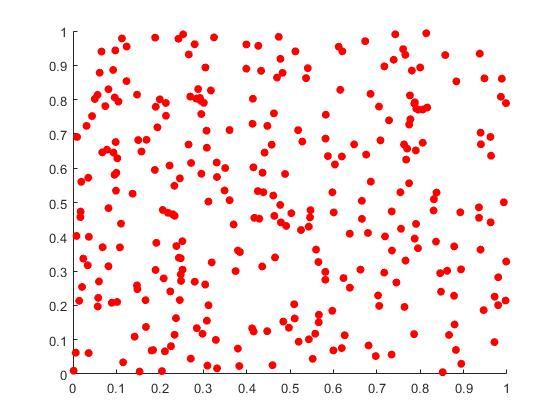
\includegraphics[scale = 0.35]{figures/init_random_pos.jpg}
    \caption{Initial Random Positions for $N = 300$ ants}
    \label{fig:initrandompos}
\end{figure}
\begin{figure}
    \centering
    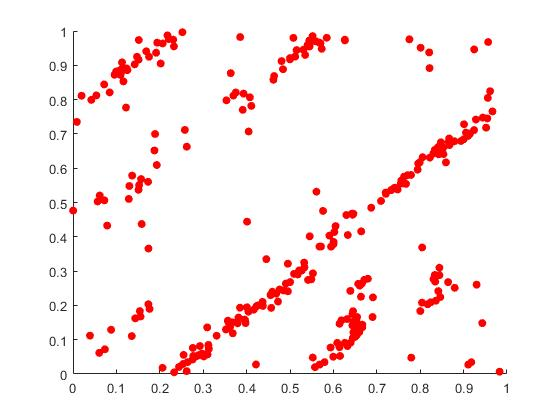
\includegraphics[scale = 0.35]{figures/final_pos_laning.jpg}
    \caption{Final ant positions after $t = 200 s$. Notice the distinctive laning formed as a result of the model}
    \label{fig:finalpos}
\end{figure}
\begin{figure}
    \centering
    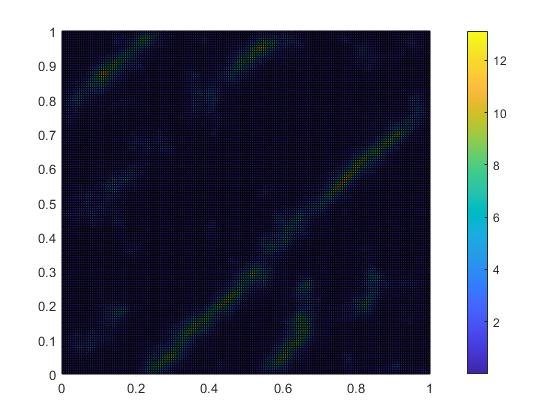
\includegraphics[scale = 0.35]{figures/conc_matrix.jpg}
    \caption{Pheromone concentration after $t = 200s$. There is a high concentration of pheromone deposited along the trails}
    \label{fig:concmatrix}
\end{figure}





\section{LCS (Lagrangian Coherent Structure) Analysis} 
\label{section:LCS}
\subsection{Background}

LCSs are surfaces of trajectories in a system that exert a major influence on nearby trajectories over time. The type of influence can vary (attracting, repelling, shearing) but they create a coherent trajectory pattern, for which the LCS can serve as a theoretical centerpiece \cite{Haller2000}.

In our case, individual ants act as the tracer particles, being carried by an underlying background flow. A \textit{dynamical system} in its most general form is -

\begin{equation}
    \left.
        \begin{array}{l}
            \dot{\vec{x}}(t;t_0,x_0) = \vec{v}(\vec{x}(t;t_0,\vec{x}_0),t) \, ,\\
            \vec{x}(t;t_0,\vec{x}_0) = \vec{x}_0 \, .
        \end{array}
    \right \}
    \label{eqn:dynamic}
\end{equation}

As time evolves, solutions of Equation \ref{eqn:dynamic} trace out curves in $D \subseteq \mathbb{R}^n$, or - they flow along their trajectory. If we fix the initial time $t_0$ and final time $t$, then we can define a flow map $\phi^t_{t_0}$ -

\begin{equation}
    \phi^t_{t_0} : D \rightarrow D : \vec{x}_0 \mapsto \phi^t_{t_0}(\vec{x}_0) = \vec{x}(t;t_0,\vec{x}_0)
\end{equation}

When analysing the phase space of these trajectories, we discover the notion of separatrices, which divide the flow into regions of distinct dynamics. For time dependent systems (as our ant model is likely to be), these separatrices themselves change with time. To find separatrices in time-dependent systems, one might look at fixed points of the instantaneous vector field and try to grow these manifolds by seeding near an instantaneous fixed point and advecting the points according to the time-dependent vector field. But separatrices in time-dependent flows aren't always connected to instantaneous fixed points, and hence we do an indirect study.

We do this by considering the behaviour of trajectories near these structures. Consider a a generic hyperbolic point and its associated stable and unstable manifolds, which is depicted in Fig. \ref{fig:hyperbolic}. If we integrate two points that are initially on either side of a stable manifold forward in time, then these points will eventually diverge from each other. Likewise, if we started two points on either side of an unstable manifold, then these points would quickly diverge from each other if integrated backward in time. This is why these manifolds are often called separatrices, since they separate trajectories which do qualitatively different things.

\begin{figure}
    \centering
    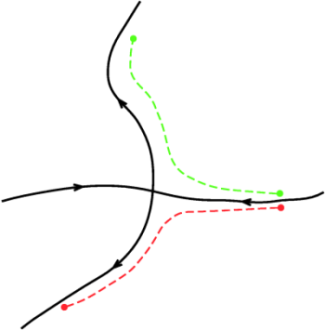
\includegraphics{figures/hyperbolic_point.png}
    \caption{Two points on either side of a separatrix will diverge from each other}
    \label{fig:hyperbolic}
\end{figure}

Therefore we take the viewpoint that since separatrices divide regions of qualitatively different dynamics, we can perhaps uncover or define such structures by looking at the divergence or stretching between trajectories. \cite{LCSTut}

\subsection{Finite-Time Lyapunov Exponents}

The finite-time Lyapunov exponent, FTLE, $\sigma_t^T(\vec{x})$, is a scalar value which characterizes the amount of stretching about the trajectory of point $\vec{x} \in D$ over the time interval $\left[t, t + T\right]$.

Consider two nearby points $\vec{x}$ and $\vec{y} = \vec{x} + \delta \vec{x}(t_0)$. After a time interval $T$, the separation between these points becomes -

\begin{align*}
    \delta \vec{x}(t_0 + T) & = \phi^{t_0 + T}_{t_0}(\vec{y}) - \phi^{t_0 + T}_{t_0}(\vec{x}) \\
    & = \frac{d\phi^{t_0 + T}_{t_0}(\vec{x})}{d\vec{x}}\delta \vec{x}(t_0) + \mathcal{O}(||\delta\vec{x}(t_0)||^2)
\end{align*}

The magnitude of perturbation is given by -

\begin{equation}
    ||\delta\vec{x}(t_0 + T)|| = \sqrt{\langle \delta\vec{x}(t_0) , \Delta \delta\vec{x}(t_0) \rangle}
\end{equation}

where, 
\begin{equation}
    \Delta = \left(\frac{d\phi^{t_0 + T}_{t_0}(\vec{x})}{d\vec{x}}\right)^*\left(\frac{d\phi^{t_0 + T}_{t_0}(\vec{x})}{d\vec{x}}\right)
\end{equation}

is a finite-time version of the Cauchy-Green deformation tensor. If we are interested in the maximum stretching occurring between points $\vec{x}$ and $\vec{y}$, we take $\delta \vec{x}(t_0)$ to be along the eigenvector associated with the maximum eigenvalue of $\Delta$. Assume $\lambda_{\text{max}}(\Delta)$ is the maximum eigenvalue, then -

\begin{equation}
    \text{max}||\delta\vec{x}(t_0 + T)|| = \sqrt{\lambda_{\text{max}}(\Delta)}||\delta\vec{x}(t_0)||
    \label{eqn:maxdelta}
\end{equation}

where $\delta\vec{x}(t_0)$ is aligned with the eigenvector described above. Define -

\begin{equation}
    \sigma_{t_0}^T(\vec{x}) = \frac{1}{|T|}\text{ln}\sqrt{\lambda_{\text{max}}(\Delta)}
\end{equation}

which makes equation \ref{eqn:maxdelta} look like 

\begin{equation}
    \text{max}||\delta\vec{x}(t_0 + T)|| = e^{\sigma_{t_0}^T(\vec{x})|T|}||\delta\vec{x}(t_0)||
\end{equation}

So, by analysing the flow of tracers placed on a uniform grid, one can obtain the FTLE associated with each point on the grid, which is what our ant simulations aim to do. FTLEs are critical in LCS analysis because separatrices are analogous to 'ridges' of high FTLE values in the FTLE field.

\subsection{FTLE fields for our model}

\begin{figure}
    \centering
    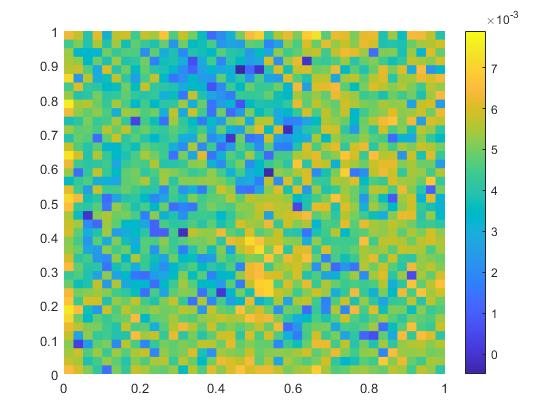
\includegraphics[scale = 0.35]{figures/FTLE_1.jpg}
    \caption{FTLE field for $t_0 = 0s, T = 20s$}
    \label{fig:ftle1}
\end{figure}

\begin{figure}
    \centering
    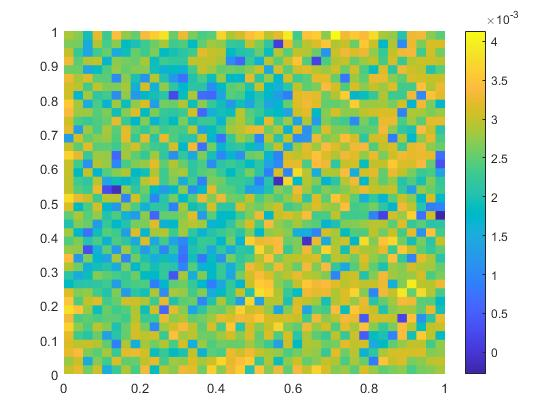
\includegraphics[scale = 0.35]{figures/FTLE_2.jpg}
    \caption{FTLE field for $t_0 = 0s, T = 40s$}
    \label{fig:ftle2}
\end{figure}

\begin{figure}
    \centering
    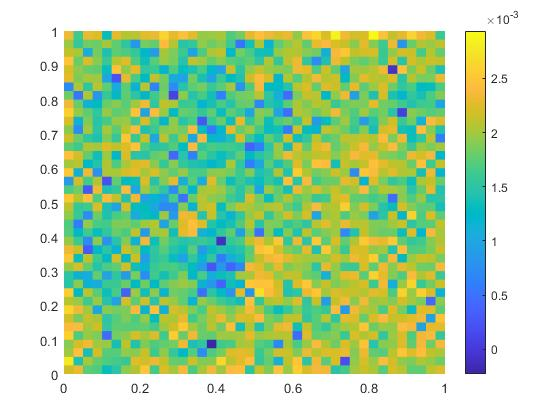
\includegraphics[scale = 0.35]{figures/FTLE_3.jpg}
    \caption{FTLE field for $t_0 = 0s, T = 60s$}
    \label{fig:ftle3}
\end{figure}

\begin{figure}
    \centering
    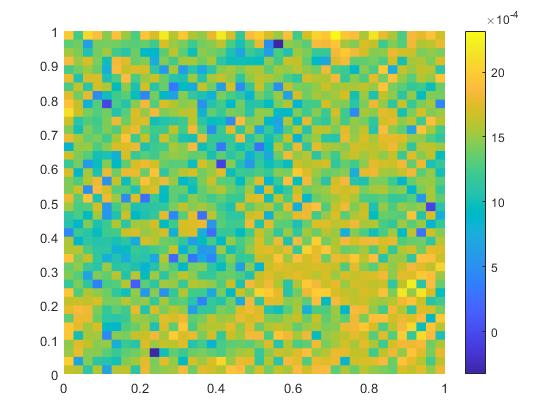
\includegraphics[scale = 0.35]{figures/FTLE_4.jpg}
    \caption{FTLE field for $t_0 = 0s, T = 80s$}
    \label{fig:ftle4}
\end{figure}

\begin{figure}
    \centering
    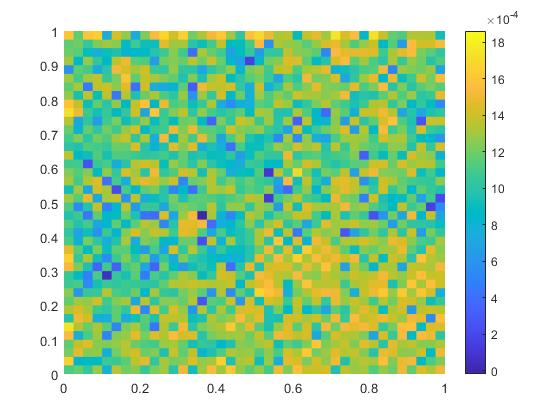
\includegraphics[scale = 0.35]{figures/FTLE_5.jpg}
    \caption{FTLE field for $t_0 = 0s, T = 100s$}
    \label{fig:ftle5}
\end{figure}

The defining characteristic of our simulations is lane formation and clumping of ants along these trails, which isn't something you readily see in the evolution of our FTLE fields. I suspect Backward-time FTLE fields will give us more stark separatrices that would correspond to our observed structures, and figuring out the best way to plot those across the entire grid is what I'm currently working on.

The figures for the FTLE fields for different values of $T$ are shown in Figures \ref{fig:ftle1}, \ref{fig:ftle2}, \ref{fig:ftle3}, \ref{fig:ftle4} and \ref{fig:ftle5}.

\section{Next Steps}
\label{sec:nextsteps}
Plotting the BFTLE fields to see if they give us more insight into the underlying velocity field governing the motion of ants is the next task. Following that, I want to experiment with different initial conditions (like pre-existing circular trails, initial conditions along pre-existing trail, etc.) to see if ant-mill formation can be replicated using the current model for these special initial conditions. 

Following these, I want to tweak the model a bit, reduce randomness, and see whether milling is a asymptotic solution to any model governing ant interaction with pheromone deposition and update defined as we already have. This would still not fully describe ant motion in isolation, since observations of ant milling claim milling to be a transient phenomena, with the mill dispersing after some time (unless the ants die of exhaustion during the mill). Observing transient vortices in the FTLE fields for certain models would also provide some insight into what the underlying velocity field for ant motion looks like.

\bibliographystyle{unsrt}
\bibliography{AntMill}

\end{document}
